\clearpage
\section{Trh výrobních faktorů (obecné a specifické výrobní faktory, produkční funkce a zákon
klesajících výnosů, poptávka a nabídka na trhu výrobních faktorů, rovnováha firmy na
trhu výrobních faktorů).}

\subsection{Obecné výrobní faktory}
\begin{itemize}
    \item Jsou to zdroje pro proces výroby.
    \item Základní skupiny:
    \begin{itemize}
        \item \textbf{práce} zahrnuje veškeré lidské zdroje, uplatnitelné ve výrobním procesu
        \item \textbf{půda} označuje v podstatě veškeré přírodní zdroje, ornou půdu, lesy, 
        zdroje nerostných surovin, moře, ovzduší apod.
        \item \textbf{kapitál} označuje výrobní faktory, které vznikají v průběhu výroby a jsou
        dále jako vstupy uplatňovány v další výrobě (suroviny, materiály, polotovary, energii, atd.)
    \end{itemize}
    \item Další obecné výrobní faktory:
    \begin{itemize}
        \item \textbf{technologie}
        \item \textbf{management}
    \end{itemize}
\end{itemize}

\subsection{Specifické výrobní faktory}
\begin{itemize}
    \item Je to konkrétní forma obecných výrobních faktorů.
    \item Např. konkrétní pozemky, kapitálové statky a pracovní profese, které jsou specializované 
    na výrobu konkrétních statků
\end{itemize}

\subsection{Produkční funkce}
\begin{itemize}
    \item Závislost produkce na množství výrobních faktorů
    \item Přírůstky produkce se nejdříve zvyšují a poté klesají.
    \item Klesá schopnost zvyšovat produkci, protože se projevuje nedostatek fixních faktorů.
    (To je \textbf{zákon klesajících výnosů})
    \item Např. produkční funkce na pile, kde je 5 strojů (fixní faktor) a variabilní počet dělníků:
\end{itemize}
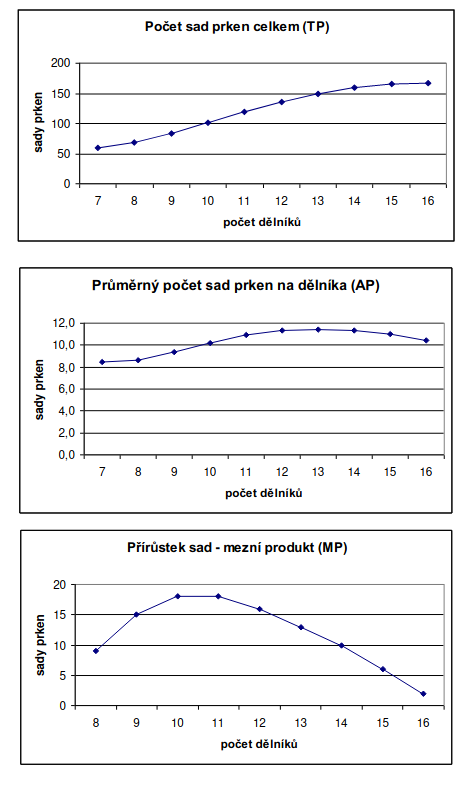
\includegraphics[]{images/16_prod_f.png}

\subsection{Poptávka na trhu výrobních faktorů}
\begin{itemize}
    \item Vůle maximalizovat zisk (největší výnosy a nejmenší náklady)
    \item Každá další jednotka výrobního faktoru:
    \begin{itemize}
        \item Mezní fyzický produkt (MP), dodatečný výstup zvýšením jednoho VF, při nezměnění ostatních
        \item Cena výrobku (P)
        \item Příjem z mezního produktu $MRP=MP\cdot P$
    \end{itemize}
\end{itemize}

\subsection{Nabídka na trhu výrobních faktorů}
\begin{itemize}
    \item Mezní náklady na výrobní faktor (MFC, Marginal Factor Costs), $MFC=\frac{\Delta TC}{\Delta VF}$,
    kde $\Delta TC$ je změna celkových nákladů a $\Delta VF$ je změna počtu výrobního faktoru
    \item Pokud panuje dokonalá konkurence, ceny výrobních faktorů udává trh a $MFC=P_F$, kde $P_F$ je
    cena za výrobní faktor
\end{itemize}

\subsection{Rovnováha firmy}
\begin{itemize}
    \item Rovnováha nastává, pokud platí $MRP=MFC$.
    \item Pokud $MRP>MFC$, firma najímá víc výrobního faktoru.
    \item Pokud $MRP<MFC$, firma snižuje nájem výrobního fkatoru.
\end{itemize}